\documentclass[catalan, a4paper, 12pt, titlepage]{article}
\usepackage{babel}
\usepackage{graphicx}
\usepackage{fontawesome5}
\graphicspath{ {../img/} }
\usepackage{mathptmx}
\renewcommand{\baselinestretch}{1.5}
%\usepackage{isolatin1}

%tikz
\usepackage{tikz}
\usetikzlibrary{mindmap}

%hyperref
\usepackage[pdftex,pdfpagelabels,bookmarks,hyperindex,hyperfigures,hidelinks]{hyperref}

\usepackage{termcal}

% Few useful commands (our classes always meet either on Monday and Wednesday
% or on Tuesday and Thursday)

\newcommand{\MWClass}{%
\calday[Monday]{\classday} % Monday
\skipday % Tuesday (no class)
\calday[Wednesday]{\classday} % Wednesday
\skipday % Thursday (no class)
\skipday % Friday
\skipday\skipday % weekend (no class)
}

\newcommand{\TRClass}{%
\skipday % Monday (no class)
\calday[Tuesday]{\classday} % Tuesday
\skipday % Wednesday (no class)
\calday[Thursday]{\classday} % Thursday
\skipday % Friday
\skipday\skipday % weekend (no class)
}

\newcommand{\MTRFClass}{%
	\calday[Monday]{\classday}
	\calday[Tuesday]{\classday}
	\skipday % Dimecres
	\calday[Thursday]{\classday}
	\calday[Friday]{\classday}
\skipday\skipday % weekend (no class)
}

\newcommand{\Holiday}[2]{%
\options{#1}{\noclassday}
\caltext{#1}{#2}
}

\usepackage{lastpage}

\usepackage{fancyhdr}

\fancyhead[L]{\small{Activitats i materials - Gestió de bases de dades}}
\fancyhead[R]{\small{Jaume Barceló Vicens}}
\fancyfoot[C]{\small{Pàgina \thepage\ de \pageref{LastPage}}}

% Uncomment to remove the header rule
\renewcommand{\headrulewidth}{0pt}

\usepackage{enumitem}
\setitemize{noitemsep,topsep=0pt,parsep=0pt,partopsep=0pt}

\usepackage{pdfpages}

\title{Activities and Materials\\ 
	\vspace{1cm}
	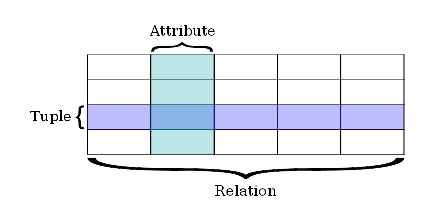
\includegraphics[width=10cm]{database.eps}
	}

\author{
	Jaume Barceló Vicens
	DNI 43135949R\\
	Professors d'ensenyament secundari (0590)
	Especialitat informàtica}

\date{
	Família professional informàtica \\
	Cicle formatiu de grau superior d’administració de sistemes informàtics en xarxa\\
	Mòdul professional de gestió de bases de dades\\
	Codi 0372 170h (+90h d'anglès)\\
	http://github.com/jbarcelo/programacio\_didactica\_gbd \\
	\faCalendar*[regular] \today %\qquad  Llicència CC-BY-SA 4.0 \faCreativeCommons\ \faCreativeCommonsBy\ \faCreativeCommonsSa
	}

\setcounter{tocdepth}{1}

\begin{document}

\pagestyle{empty}

\maketitle

\tableofcontents

\newpage

\pagestyle{fancy}

\section{Unit 1: Introduction}

%\includepdf[pages=-, nup=2x2]{activities/unit01/01_01_Slides_1-1_Introduction_to_databases.pdf}
\includepdf[pages=-]{activities/unit01/01_02_Assignment_1-1_Introduction_to_databases.pdf}
\includepdf[pages=-]{activities/unit01/01_03_Assignment_1-2_The_Role_of_a_DBA.pdf}
\includepdf[pages=-]{activities/unit01/01_04_Test_Introduction_to_databases.pdf}

\section{Unit 2: Introduction to the Relational Model}

%\includepdf[pages=-, nup=2x2]{activities/unit02/02_01_Slides_2-1_Relational_Model.pdf}
\includepdf[pages=-]{activities/unit02/02_02_Assignment_2-1_Install_a_DBMS.pdf}
\includepdf[pages=-]{activities/unit02/02_03_Assignment_2-2_Keys.pdf}
\includepdf[pages=-]{activities/unit02/02_04_Assignment_2-3_Relational_Diagram.pdf}
\includepdf[pages=-]{activities/unit02/02_05_Assignment_2-4_Relational_Algebra.pdf}
\includepdf[pages=-]{activities/unit02/02_06_Test_Introduction_to_the_Relational_Model.pdf}

\section{Unit 3: Introduction to SQL 1}

%\includepdf[pages=-, nup=2x2]{activities/unit03/03_01_Slides_3-1_Introduction_to_SQL.pdf}
\includepdf[pages=-]{activities/unit03/03_02_Assignment_3-1_Create_a_Database.pdf}
\includepdf[pages=-]{activities/unit03/03_03_Assignment_3-2_Dockerized_Database.pdf}
\includepdf[pages=-]{activities/unit03/03_03_Assignment_3-2_Dockerized_Database_guia_professor.pdf}
\includepdf[pages=-]{activities/unit03/03_04_Assignment_3-3_School_Database_Script.pdf}
\includepdf[pages=-]{activities/unit03/03_05_Material_3-1_Requirements_for_the_Test.pdf}
\includepdf[pages=-]{activities/unit03/03_06_Test_Introduction_to_SQL.pdf}

\section{Unit 4: Introduction to SQL 2}

%\includepdf[pages=-, nup=2x2]{activities/unit04/04_01_Slides_4-1_Introduction_to_SQL_2.pdf}
\includepdf[pages=-]{activities/unit04/04_02_Material_4-1_Queries_MariaDB.pdf}
\includepdf[pages=-]{activities/unit04/04_03_Material_4-2_Queries_MariaDB.pdf}
\includepdf[pages=-]{activities/unit04/04_04_Material_4-3_Northwind.pdf}
\includepdf[pages=-]{activities/unit04/04_05_Test_Introduction_to_SQL_2.pdf}

\section{Unit 5: Intermediate SQL 1}

%\includepdf[pages=-, nup=2x2]{activities/unit05/05_01_Slides_5-1_Intermediate_SQL_1.pdf}
\includepdf[pages=-]{activities/unit05/05_02_Assignment_5-1_Dockerized_phpMyAdmin_in_Google_CloudShell.pdf}
\includepdf[pages=-]{activities/unit05/05_03_Material_5-1_Join.pdf}
\includepdf[pages=-]{activities/unit05/05_04_Material_5-2_View.pdf}
\includepdf[pages=-]{activities/unit05/05_05_Material_5-3_Transactions_1.pdf}
\includepdf[pages=-]{activities/unit05/05_06_Material_5-4_Transactions_2.pdf}
\includepdf[pages=-]{activities/unit05/05_07_Assignment_5-2_Two-Phase_Locking_and_Snapshop_Isolation.pdf}
\includepdf[pages=-]{activities/unit05/05_08_Test_Intermediate_SQL_1.pdf}

\section{Unit 6: Intermediate SQL 2}

%\includepdf[pages=-, nup=2x2]{activities/unit06/06_01_Slides_6-1_Intermediate_SQL_2.pdf}
\includepdf[pages=-]{activities/unit06/06_02_Material_6-1_Referential_Integrity_and_Data_Types.pdf}
\includepdf[pages=-]{activities/unit06/06_03_Assignment_6-1_Mini-league.pdf}
\includepdf[pages=-]{activities/unit06/06_04_Material_6-2_Index_Importance.pdf}
\includepdf[pages=-]{activities/unit06/06_05_Material_6-3_Authorization.pdf}
\includepdf[pages=-]{activities/unit06/06_06_Material_6-4_Roles.pdf}
\includepdf[pages=-]{activities/unit06/06_07_Material_6-5_Dates.pdf}
\includepdf[pages=-]{activities/unit06/06_08_Test_Intermediate_SQL_2.pdf}

\section{Unit 7: Advanced SQL 1}

\includepdf[pages=-]{activities/unit07/07_01_Material_7-1_SQL_Statements_in_a_Java_Application.pdf}
\includepdf[pages=-]{activities/unit07/07_02_Assignment_7-1_JDBC_Project.pdf}
\includepdf[pages=-]{activities/unit07/07_03_Assignment_7-2_Video_Explanation_Demonstration.pdf}

\section{Unit 8: Advanced SQL 2}

\includepdf[pages=-]{activities/unit08/08_01_Material_8-1_Postgres.pdf}
\includepdf[pages=-]{activities/unit08/08_02_Material_8-2_PostgreSQL_PL_pgSQL.pdf}
\includepdf[pages=-]{activities/unit08/08_03_Assignment_8-1_Create_a_Function.pdf}
\includepdf[pages=-]{activities/unit08/08_04_Assignment_8-2_Present_and_Defend_Your_Functions.pdf}
\includepdf[pages=-]{activities/unit08/08_05_Assignment_8-3_Create_a_Cursor_a_Stored_Procedure_and_a_Trigger.pdf}
\includepdf[pages=-]{activities/unit08/08_06_Assignment_8-4_Present_and_Defend_Your_Cursor_Trigger_Procedure.pdf}

\section{Unit 9: Database Design and the E-R Model}

%\includepdf[pages=-, nup=2x2]{activities/unit09/09_01_Slides_9-1_Database_Design_and_the_E-R_Model.pdf}
\includepdf[pages=-]{activities/unit09/09_02_Material_9-1_E-R_Diagram_Tool.pdf}
\includepdf[pages=-]{activities/unit09/09_03_Material_9-2_E-R_exercises.pdf}
\includepdf[pages=-]{activities/unit09/09_04_Assignment_9-1_Create_an_ERD.pdf}
\includepdf[pages=-]{activities/unit09/09_05_Assignment_9-2_Defend_Your_ERD.pdf}

\section{Unit 10: Database Design. E-R Model to Relational Model}

%\includepdf[pages=-, nup=2x2]{activities/unit10/10_01_Slides_10-1_Database_Design_E-R_Model_to_Relational_Model.pdf}
\includepdf[pages=-]{activities/unit10/10_02_Material_10-1_E-R_to_Relational_Exercises.pdf}
\includepdf[pages=-]{activities/unit10/10_03_Assignment_10-1_ERM_to_Relational_Model.pdf}
\includepdf[pages=-]{activities/unit10/10_04_Assignment_10-2_Defend_Your_ERM_to_Relational_Model.pdf}

\section{Unit 11: Database Design. Normalization}

\includepdf[pages=-]{activities/unit11/11_01_Slides_11-1_Normalization.pdf}
%\includepdf[pages=-, nup=2x2]{activities/unit11/11_02_Slides_11-2_Normalization.pdf}
\includepdf[pages=-]{activities/unit11/11_03_Material_11-1_Normalization_Exercises.pdf}
\includepdf[pages=-]{activities/unit11/11_04_Material_11-2_Example_of_Solution.pdf}
\includepdf[pages=-]{activities/unit11/11_05_Assignment_11-1_Normalization.pdf}
\includepdf[pages=-]{activities/unit11/11_06_Assignment_11-2_Present_Your_Normalization.pdf}

\section{Unit 12: Advanced Topics}

\includepdf[pages=-]{activities/unit12/12_01_Assignment_12-1_Advanced_Topics.pdf}
\includepdf[pages=-]{activities/unit12/12_02_Material_12-1_NoSQL.pdf}

\section{Google Classroom}
\includepdf[pages=-]{activities/classroom/exemple_classroom_dual.pdf}

\end{document}
